\documentclass{beamer}
\usepackage[utf8]{inputenc}
\usepackage{textcomp}  % Required for encoding \textbigcircle
\usepackage{scalerel}  % Required for emoji \scalerel
\usepackage{enumitem}
\usepackage{listings}
\usepackage{textcomp}
\usepackage{lmodern}
\usepackage{caption}
\usepackage{svg}

\usepackage[T1]{fontenc}
\renewcommand*\oldstylenums[1]{{\fontfamily{Montserrat-TOsF}\selectfont #1}}

\def\tada{\scalerel*{
\includegraphics{img/1f389.eps}}{\textrm{\textbigcircle}}}

\usetheme{Madrid}
\definecolor{theme}{rgb}{0.06274509803921569, 0.18823529411764706, 0.21568627450980393}

\useoutertheme{infolines} % Alternatively: miniframes, infolines, split
\useinnertheme{circles}
\usecolortheme[named=theme]{structure}

\lstset{basicstyle=\footnotesize\ttfamily,breaklines=true}

%------------------------------------------------------------
%This block of code defines the information to appear in the
%Title page
\title[Leveraging Machine Interpretability]{Interpretability Tools as Feedback Loops}

\subtitle{BoilerMake X}

\author{J.~Setpal}

\date{January 21, 2023}

\titlegraphic{\includegraphics[width=7cm]{img/logo-full.png}}


%End of title page configuration block
%------------------------------------------------------------



%------------------------------------------------------------
%The next block of commands puts the table of contents at the 
%beginning of each section and highlights the current section:

\AtBeginSection[]
{
  \begin{frame}
    \frametitle{Outline}
    \tableofcontents[currentsection]
  \end{frame}
}
% ------------------------------------------------------------


\begin{document}

%The next statement creates the title page.
\frame{\titlepage}

\logo{\includegraphics[width=2.5cm]{img/logo-full.png}}

%---------------------------------------------------------
% This block of code is for the table of contents after
% the title page
\begin{frame}
\frametitle{Outline}
\tableofcontents
\end{frame}
%---------------------------------------------------------

\section{Setting the Stage}
\begin{frame}[fragile]{Here's a Scenario}
	Consider the following:
	\begin{enumerate}[label=\alph*.]
		\item We want to build a classifier (classifiers are cool). \pause
		\item This classifier differentiates between an Orca and a Leopard. \pause
		\item We use the \href{https://data.caltech.edu/records/nyy15-4j048}{Caltech-256} dataset to obtain images of both:
			\begin{center}
				\hspace*{-2em}  
				\includegraphics[width=\textwidth]{img/dataset.pdf}
			\end{center} \pause 
		\item There are \texttt{188} leopard images and 89 orca images.
	\end{enumerate} 
\end{frame}

\begin{frame}{More Scenario Stuff}
	Here's our model architecture:
	\begin{center}
		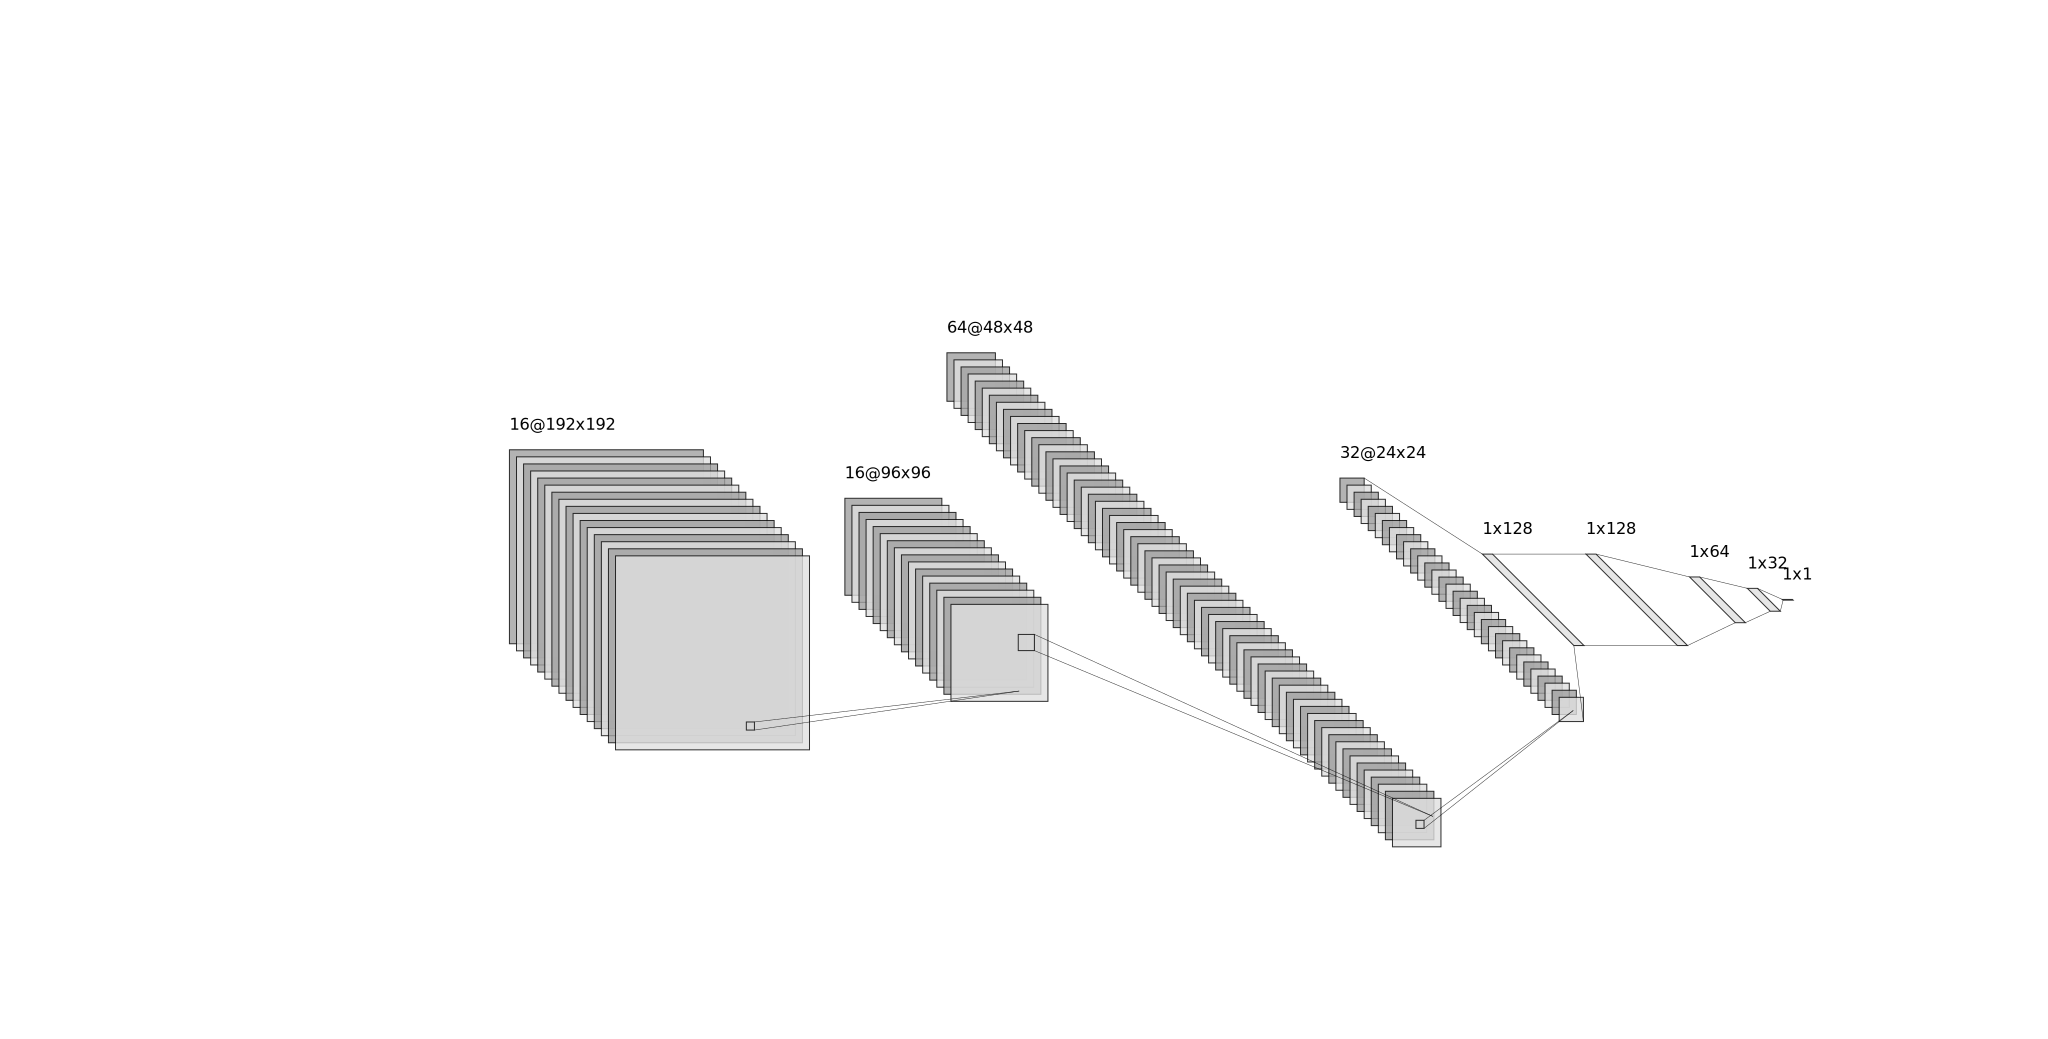
\includegraphics[width=\textwidth]{img/nn}
	\end{center}
\end{frame}

\begin{frame}{Last Bit of Scenario, I Promise}
	We use:
	\begin{enumerate}[label=\alph*.]
		\item Optimizer: \texttt{SGD}
			\begin{enumerate}[label=-]
				\item Learning Rate: $10^{-2}$
				\item Epsilon: $10^{-8}$
			\end{enumerate}
		\item Loss: \texttt{BinaryCrossEntropy}
		\item Epochs: 5
	\end{enumerate} \pause
	During training, our training and validation accuracies are $\approx$ \texttt{1.000} \tada \pause \\
	However, we achieve a \textbf{test accuracy} of only \texttt{0.5938}. This \textit{sucks}. \pause \\

	Here are some misclassified samples:
	\begin{center}
		\hspace*{-7em}
		\includegraphics[width=10cm]{img/misclassifications}
	\end{center}
\end{frame}

\section{Baselining Interpretability}

\begin{frame}{What even \textit{is} Interpretability?}
	\begin{columns}
		\begin{column}{0.5\textwidth}
			\begin{center}
				\includegraphics[width=5cm]{img/1838} \pause
			\end{center}
		\end{column}
		\begin{column}{0.5\textwidth}
			Interpretability within Machine Learning is the \textbf{degree} to which we can understand the \textbf{cause} of a decision, and use it to consistently \underline{predict the model's prediction}. \pause \newline \\

			This is easy for shallow learning. \pause For deep learning however, it is a \textbf{lot harder}.
		\end{column}
	\end{columns}
\end{frame}

\begin{frame}{A Cautionary Tale}
	Let's explore: \url{https://interaktiv.br.de/ki-bewerbung/en/} \newline \\

	Start-up attempting to make the application process `faster, but also more objective and fair'. \pause \newline \\
	They were not successful.
\end{frame}

\begin{frame}{Class Activation Mappings}
	For deep learning, interpretability techniques today involve a fairly straightforward formula: \pause
	\begin{enumerate}[label=-]
		\item Split hidden layers.
		\item Expose weights.
		\item \textit{Observe!} \pause
	\end{enumerate}
	We'll focus today's discussion on \textbf{Class Activation Mappings (CAMs)}:
	\vspace{1em} \includegraphics[width=9.5cm]{img/cams}
\end{frame}

\begin{frame}{Building Feedback Loops}
	Finding optimal model weights is an \textbf{NP-hard} problem. \pause \\
	\begin{columns}
		\begin{column}{.5\textwidth}
			\begin{figure}
				\includegraphics[width=4.5cm]{img/np}
				\caption*{\footnotesize Model Search Space}
			\end{figure} \pause
		\end{column}
		\begin{column}{.5\textwidth}
			We can't speed this up. However, we do have information about our training set that we can use to \textbf{motivate training behaviour}. \pause \newline \\
		\end{column}
	\end{columns}
	So, the idea here is simple: use \underline{shared knowledge} (+ common sense) to modify how we train our models.
\end{frame}

\begin{frame}{Updating the Search Space}
	We approach the challenge in the \textit{opposite} direction. \pause Instead of optimizing how we solve the search space, let's \textbf{update the search space} itself! \pause \newline \\

	\begin{columns}
		\begin{column}{.3\textwidth}
			\begin{figure}
				\includegraphics[width=4.5cm]{img/space.png}
				\caption*{\footnotesize Updated Search Space!}
			\end{figure}
		\end{column}
		\begin{column}{.5\textwidth}
			By updating our loss function to eliminate \textit{pseudo-correctness}, we can: \pause
			\begin{enumerate}[label=-]
				\item Make the optimal weights incredibly easy for our optimzer to find. \pause
				\item Allow our generalized model to \underline{extrapolate on implicit information}.
			\end{enumerate}
		\end{column}
	\end{columns}
\end{frame}

\section{Leveraging Interpretability}
\begin{frame}{Getting Back to the Challenge}
	There are some obvious causes for why it performs poorly:
	\begin{enumerate}[label=\alph*.]
		\item There are too few, unbalanced training samples. \pause \\
			\underline{Solution:} Data Augmentation / Covariate Shift \pause
		\item \textbf{The images have a sharp color dominance.} \pause
			\begin{center}
				\vspace{-1em}
				\hspace*{-2em}  
				\includegraphics[width=\textwidth]{img/dataset.pdf}
			\end{center}
	\end{enumerate}
\end{frame}

\begin{frame}{Diagnosing the Model}
	When we obtain a Class Activation Map of a sample image, we observe:
	\begin{center}
		\vspace{-.8em}
		\includegraphics[width=8cm]{img/bad-cam}
	\end{center} \pause
	\vspace{-1em}
	It \textbf{does not} use the leopard to base it's prediction!
	This is prevalent \underline{across the dataset}. \pause \newline \\

	\textbf{Observation:} The targets in our entire training dataset are centered. \pause \newline \\

	Q: Can we exploit this?
\end{frame}

\begin{frame}{Exploiting a Centred Dataset}
	Idea: Let's penalize our batch whenever the CAM is off-center. \pause \newline \\

	We can achieve this by inverting a 2D Gaussian Kernel.
	\begin{columns}
		\begin{column}{.4\textwidth}
			\begin{figure}
				\includegraphics[width=\textwidth]{img/kernel}
				\caption*{\footnotesize Inverted Gaussian Kernel}
			\end{figure} \pause
		\end{column}
		\begin{column}{.6\textwidth}
			Weights scale sharply as the operation approaches the image boundary. \pause \newline \\

			It has to \underline{not} be perfect, since we don't intend to overfit our model to this setup. This kernel filter is a \textbf{guideline}.
		\end{column}
	\end{columns}
\end{frame}

\begin{frame}{Introducing \texttt{CAMLoss}!}
	Here's how it all comes together: 
	\begin{enumerate}[label=\alph*.]
		\item In addition to the prediction, we output the class activation map. \pause
		\item We apply our kernel filter on every batch. \pause
		\item We return the mean of the returned features. Weights $\propto \frac{1}{\text{Fit Quality}}$ \pause
		\item This is our additional self-supervised loss function! \pause
	\end{enumerate}
	Obtaining the Class Activation Map of the updated model, we observe:
	\begin{center}
		\vspace{-.9em}
		\includegraphics[width=10cm]{img/fixed-cam}
	\end{center} \pause
	\vspace{-1em}
	\textbf{Great Success!}
\end{frame}

\begin{frame}{Implementation Details}
	\begin{center}
                If you can view this screen, I am making a mistake.
        \end{center}
\end{frame}

\begin{frame}{Thank you!}
	\begin{center}
		Have an awesome rest of your day! Any questions for me?
	\end{center}
	\begin{center}
		\textbf{Code, Experiments, Data, Slides:} \url{https://dagshub.com/jinensetpal/lint.git}
	\end{center}
\end{frame}

\end{document}
